\documentclass[a4paper,14pt]{extarticle}

\usepackage{iftex}
\usepackage{geometry}
\ifPDFTeX
\usepackage[T2A]{fontenc}
\usepackage[utf8]{inputenc}
\usepackage[english,russian]{babel}
\usepackage{tempora}
\else
\usepackage{fontspec}
\usepackage{polyglossia}
\setdefaultlanguage{russian}
\setotherlanguage{english}
\setmainfont{Times New Roman}
\setsansfont{Arial}
\setmonofont{Courier New}
\newfontfamily\cyrillicfonttt{Times New Roman}
\fi
\usepackage{amsmath}
\usepackage{amsthm}
\usepackage{amssymb}
\usepackage{mathtools}
\usepackage{fancyhdr}
\usepackage{setspace}
\usepackage{graphicx}
\usepackage{colortbl}
\usepackage{tikz}
\usepackage{pgf}
\usepackage{subcaption}
\usepackage{listings}
\usepackage{indentfirst}
\usepackage{booktabs}
\usepackage{float}
\usepackage[flushleft]{threeparttable}
\usepackage{tablefootnote}
\usepackage{tabularx}
\usepackage{array}
\usepackage{caption}
\usepackage{enumitem}
\usepackage{chngcntr}
\usepackage{xurl}
\usepackage{csquotes}
\usepackage[
backend=biber,
style=numeric,
maxbibnames=99,
sorting=none
]{biblatex}
\addbibresource{refs.bib}
\usepackage[hidelinks,bookmarks=false,hypertexnames=true]{hyperref}


\counterwithin{table}{section}
\counterwithin{figure}{section}

\graphicspath{{graphics/}}

\geometry{left=2.5cm}
\geometry{right=1.0cm}
\geometry{top=2.0cm}
\geometry{bottom=2.0cm}
\setlength{\parindent}{1.25cm}
\renewcommand{\baselinestretch}{1.5}
\setlength{\textfloatsep}{12pt plus 2pt minus 2pt}
\setlength{\floatsep}{10pt plus 2pt minus 2pt}
\setlength{\intextsep}{10pt plus 2pt minus 2pt}
\setlength{\abovecaptionskip}{6pt}
\setlength{\belowcaptionskip}{6pt}
\setlist[enumerate]{itemsep=0.2em,topsep=0.2em}
\emergencystretch=2em
\Urlmuskip=0mu plus 1mu\relax

\fancyhf{}
\fancyfoot[C]{\thepage}
\renewcommand{\headrulewidth}{0pt}
\renewcommand{\footrulewidth}{0pt}
\pagestyle{fancy}

\DeclareCaptionFont{tablefont}{\fontsize{12}{14}\selectfont}
\captionsetup[table]{font=tablefont}

\renewcommand{\labelenumi}{\arabic{enumi}.}
\renewcommand{\labelenumii}{\arabic{enumi}.\arabic{enumii}.}
\renewcommand{\labelenumiii}{\arabic{enumi}.\arabic{enumii}.\arabic{enumiii}.}

\DefineBibliographyStrings{russian}{
    bibliography = {Список литературы}
}

\begin{document}

	\begin{titlepage}
		\thispagestyle{empty}
		{\setstretch{1.0}
			\begin{center}
				{\bfseries
				ФЕДЕРАЛЬНОЕ ГОСУДАРСТВЕННОЕ АВТОНОМНОЕ ОБРАЗОВАТЕЛЬНОЕ\\
				УЧРЕЖДЕНИЕ ВЫСШЕГО ОБРАЗОВАНИЯ\\
				<<НАЦИОНАЛЬНЫЙ ИССЛЕДОВАТЕЛЬСКИЙ УНИВЕРСИТЕТ\\
				<<ВЫСШАЯ ШКОЛА ЭКОНОМИКИ>>\\
				ФАКУЛЬТЕТ КОМПЬЮТЕРНЫХ НАУК}
			\end{center}
			
			\vspace{1.0cm}
			
			\begin{center}
				{Кузнецов Егор Сергеевич}
			\end{center}

			\vspace{1.0cm}

			\begin{center}
				МАГИСТЕРСКАЯ ДИССЕРТАЦИЯ
			\end{center}

			\vspace{0.8cm}

			\begin{center}
				\begin{minipage}{0.96\textwidth}
					\centering
					\setstretch{1.05}
					{\textbf{Разработка алгоритма распознавания показаний круглых аналоговых шкал на изображениях с применением глубокого обучения}}\\[0.35em]
					{\textbf{Development of an Algorithm for Recognizing Readings of Round Analog Scales in Images Using Deep Learning}}
				\end{minipage}
			\end{center}

			\vspace{0.8cm}

			\begin{center}
				по направлению подготовки 01.04.02 Прикладная математика и информатика\\
				образовательная программа <<Искусственный интеллект>>
			\end{center}

			\vspace{1.0cm}

			\noindent
			\begin{minipage}[t]{0.42\textwidth}
				Студент\\
				Е.\,С. Кузнецов
			\end{minipage}

			\vspace{1.0cm}

			\noindent
			\hfill
			\begin{minipage}[t]{0.58\textwidth}
				\raggedleft
				Научный руководитель\\
				доцент\\
				И.\,А. Макаров
			\end{minipage}

			\vfill

			\begin{center}
				Москва 2026
			\end{center}
		}

	\end{titlepage}

		\setcounter{page}{2}

		\hypersetup{linkcolor=black}
		\begin{spacing}{1.0}
		\tableofcontents
		\end{spacing}
		\hypersetup{linkcolor=blue}

	\newpage

\section*{Аннотация}
\begingroup
\fontsize{13.4}{16}\selectfont
ВКР посвящена распознаванию показаний круглых аналоговых шкал по изображению. Такая постановка остается практичной для производственных объектов, где исправные стрелочные приборы уже встроены в технологический процесс, а их замена на цифровые датчики требует остановки оборудования и дополнительных работ по интеграции. Поэтому в работе рассматривается не замена измерительного контура, а визуальный слой считывания: камера фиксирует установленный прибор, а алгоритм переводит положение стрелки в численное значение.

Эксперименты проведены на наборе SynthGauge и построены вокруг трех вариантов решения: детекции прибора с ключевыми точками шкалы, геометрического контура с сегментацией стрелки и прямой регрессии нормализованного показания. Сравнение показало, что найти циферблат на синтетических изображениях удается почти безошибочно, но итоговая ошибка определяется более тонкими этапами: положением центра, границами шкалы и качеством маски стрелки. ResNet-18 дает лучший результат на синтетическом тесте, однако геометрический пайплайн удобнее для диагностики, потому что показывает, где именно возник сбой. Проверка на реальных фотографиях выявила заметный доменный разрыв; поэтому текущий результат следует рассматривать как воспроизводимый экспериментальный контур и основу для дальнейшей адаптации под конкретные приборы.
\endgroup

	\addcontentsline{toc}{section}{Аннотация}

	\section*{Ключевые слова}
	\vspace{-0.7em}
	аналоговые датчики, компьютерное зрение, считывание показаний, синтетические данные, детекция объектов, ключевые точки, сегментация стрелки, регрессия

		\addcontentsline{toc}{section}{Ключевые слова}

		\newpage
\section*{Abstract}
\begingroup
\fontsize{13.4}{16}\selectfont
This thesis focuses on recognizing readings of round analog scales from images. This setting remains practical for production facilities where working pointer gauges are already embedded into the technological process, while replacing them with digital sensors requires equipment downtime and additional integration work. Therefore, the thesis considers not a replacement of the measurement loop, but a visual reading layer: a camera observes an installed gauge, and the algorithm converts the needle position into a numerical value.

The experiments are based on the SynthGauge dataset and compare three solution variants: gauge detection with scale keypoints, a geometric pipeline with needle segmentation, and direct regression of the normalized reading. The comparison shows that dial detection on synthetic images is almost error-free, while the final error is determined by finer stages: the center position, scale boundaries, and the quality of the needle mask. ResNet-18 achieves the best result on the synthetic test set, but the geometric pipeline is more convenient for diagnostics because it shows where the failure occurred. Testing on real photographs reveals a noticeable domain gap; therefore, the current result should be treated as a reproducible experimental pipeline and a basis for further adaptation to specific gauges.
\endgroup

		\addcontentsline{toc}{section}{Abstract}

		\section*{Keywords}
		\vspace{-0.7em}
		analog gauges, computer vision, gauge reading, synthetic data, object detection, keypoints, needle segmentation, regression

		\addcontentsline{toc}{section}{Keywords}

		\newpage
	\section{Введение}

Автоматическое считывание показаний аналоговых стрелочных приборов остается актуальной задачей для промышленности, энергетики, транспорта и систем технического мониторинга. Несмотря на распространение цифровых датчиков, на реальных объектах по-прежнему используется большое число аналоговых манометров, амперметров, вольтметров и других приборов, показания которых часто снимаются вручную. Это делает задачу автоматического распознавания практической и исследовательской одновременно \cite{schuetze2018,adsul2021,howells2021,reitsma2024}.

Особенно заметна эта проблема на малых и средних производствах. Для крупного предприятия цифровизация измерительной инфраструктуры может быть частью долгосрочной программы модернизации: датчики заменяются на цифровые, данные поступают в SCADA или MES-системы, а технологические процессы постепенно перестраиваются под новые каналы мониторинга. Для небольшого завода такой путь часто оказывается слишком дорогим. Стоимость самих датчиков является только одной частью затрат: дополнительно нужны монтаж, остановка оборудования, перенастройка автоматики, проверка совместимости с существующими контроллерами, обучение персонала и последующее обслуживание.

Поэтому на практике большое количество исправных аналоговых приборов продолжает использоваться даже тогда, когда руководству предприятия уже нужны цифровые журналы, контроль отклонений и удаленный мониторинг. Компьютерное зрение в таком сценарии не заменяет промышленную автоматизацию полностью, но позволяет сделать более мягкий переход. Камера может быть установлена перед существующим прибором, а алгоритм считывания будет переводить визуальное показание в числовое значение. Такое решение не требует вмешательства в измерительный контур, не меняет сертифицированную часть оборудования и может внедряться постепенно: сначала для контроля отдельных узких мест, затем для расширения мониторинга на другие участки.

Со стороны компьютерного зрения эта задача сложнее обычной классификации. Необходимо найти прибор в кадре, определить положение стрелки относительно шкалы и перевести геометрию изображения в числовое значение. Дополнительные трудности создают блики, загрязнения, искажение перспективы и разнообразие конструкций приборов \cite{howells2021,wang2022,reitsma2024,coords2023,sciRep2025}.

Еще одна проблема связана с нехваткой публичных размеченных данных. Для таких систем важную роль играют синтетические наборы данных и доменная рандомизация, позволяющие получать большие объемы автоматически размеченных изображений и воспроизводимо сравнивать модели \cite{leon2024,tobin2017,horvath2023,blenderproc2020,zhang2019,syntheticReview2022}.

В данной работе поиск оптимального решения осуществляется на наборе SynthGauge. В практической части сравниваются два семейства подходов: интерпретируемый геометрический пайплайн, в котором детекция циферблата, локализация ключевых точек и сегментация стрелки образуют единый контур считывания, и прямая регрессия нормализованного показания \cite{howells2021,leon2024,reitsma2024,sciRep2025,meterRegression2024}.

	Целью работы является анализ и сравнение методов автоматического считывания показаний аналоговых стрелочных датчиков по изображениям на основе синтетических данных и единого экспериментального контура.

	Для достижения поставленной цели формулируются следующие задачи:

\begin{enumerate}[leftmargin=1.5cm]
	\item Проанализировать специфику задачи считывания показаний аналоговых приборов и основные трудности ее автоматизации.
	\item Рассмотреть существующие подходы: геометрические методы, локализацию ключевых точек, сегментацию стрелки и прямую регрессию.
	\item Описать экспериментальный контур на базе набора SynthGauge и используемые метрики качества.
	\item Описать алгоритм восстановления угла стрелки и перевода угловой геометрии в нормализованное показание.
	\item Сравнить интерпретируемый пайплайн, прямую регрессию и проверку на реальных изображениях, определить ограничения текущего решения и направления его развития.
\end{enumerate}

	Объектом исследования являются изображения аналоговых стрелочных приборов промышленного типа.

	Предмет исследования составляют методы компьютерного зрения и машинного обучения, применяемые для локализации прибора, оценки геометрии стрелки и шкалы, а также для прямого предсказания отображаемого числового значения.

	Научная новизна работы состоит в систематическом сопоставлении различных формализаций одной и той же прикладной задачи на едином наборе синтетических данных с общей схемой аннотаций. Такой подход позволяет более четко понять, в каком месте задачи возникает основная ошибка: на этапе обнаружения прибора, на этапе восстановления его геометрии или на этапе прямого вычисления показания.

	Методы исследования включают анализ существующих подходов компьютерного зрения, подготовку данных в форматах детекции, локализации ключевых точек, сегментации и регрессии, обучение моделей на синтетическом наборе SynthGauge, расчет метрик качества для отдельных этапов и сравнительный анализ итоговой ошибки считывания.

	Практическая значимость работы связана с возможностью использования разработанного пайплайна как основы для систем дистанционного промышленного мониторинга. Для малых предприятий такой подход особенно полезен как вариант постепенной цифровизации: вместо немедленной замены всей приборной базы можно добавить визуальный слой контроля поверх уже установленного оборудования. Полученные результаты могут быть использованы при проектировании сервисов автоматической инспекции оборудования, а также как база для дальнейшего перехода от синтетического домена к реальным производственным изображениям.

	В данной работе сначала рассматриваются существующие подходы, синтетические данные и метрики оценки, затем описываются данные, эксперименты, анализ результатов и итоговые выводы.

	\newpage
	\section{Теоретическая часть}

	\subsection{Специфика задачи считывания показаний аналоговых датчиков}

Задача считывания показаний аналогового стрелочного прибора по изображению состоит из последовательного решения трех подзадач: локализация объекта, восстановление геометрии шкалы и стрелки и перевод геометрии в число. В отличие от обычной классификации, здесь важна не только принадлежность изображения к классу, но и точное взаимное расположение визуальных элементов \cite{howells2021,wang2022,reitsma2024,coords2023}.

Сложность усиливается из-за высокой вариативности приборов и условий съемки. На результат влияют форма корпуса, тип шкалы, материал стекла, блики, загрязнения, перспектива и частичное перекрытие. Поэтому даже небольшая ошибка в положении стрелки может приводить к заметной ошибке итогового показания \cite{dyer1983,adsul2021,coords2023,sciRep2025}.

С прикладной точки зрения качество алгоритма нельзя отделять от способа его внедрения. На небольшом производстве стрелочный манометр или амперметр часто является не отдельной деталью, а частью уже согласованной схемы: рядом находятся трубопровод, электрическая обвязка, шкаф автоматики, регламент поверки и инструкции для персонала. Замена такого прибора на цифровой датчик может потребовать остановки участка и повторной проверки всей цепочки измерения. По этой причине вариант с внешней камерой ценен сам по себе: он добавляет цифровое наблюдение, но не заставляет сразу перестраивать оборудование.

Визуальное считывание хорошо подходит для такого постепенного сценария. На первом этапе система может просто фиксировать показания в журнале или подсказывать оператору значение, затем использоваться для сигналов о выходе за допустимый диапазон, а уже после накопления реальных данных переходить к более строгому контролю. Поэтому задача интересна не только как компьютерное зрение на синтетическом наборе, но и как инженерный компромисс для предприятий, где стоимость простоя важнее стоимости отдельного датчика.

	\subsection{Основные подходы к решению задачи}

Исторически задачи считывания стрелочных приборов решались геометрическими и эвристическими методами: через поиск окружности циферблата, выделение стрелки, оценку угла и перевод этого угла в показание. Для этого применялись преобразование Хафа, анализ контуров, бинаризация и морфологические операции. Такие методы интерпретируемы, но чувствительны к качеству изображения и отклонениям реальной геометрии от ожидаемой модели \cite{hassanein2015,incrementalHough2016,dyer1983,coords2023,kudrina2014}.

Современные подходы чаще опираются на глубокое обучение. В рамках данной работы важны три практические схемы. Первая схема является интерпретируемой: прибор сначала детектируется на изображении, а затем на уже вырезанном участке со шкалой детектируются центр шкалы, ее границы и кончик стрелки. Вторая схема заменяет детекцию кончика на сегментацию стрелки, то есть модель выделяет не одну точку, а всю область указателя. Третья схема сразу предсказывает показание по изображению циферблата и тем самым упрощает контур, но делает его менее прозрачным для анализа ошибок \cite{yoloSurvey2022,howells2021,reitsma2024,leon2024,meterRegression2024,sciRep2025,deng2022,peng2024,linknetYolo2024}.

	\subsection{Сегментация стрелки как промежуточное представление}

	Ключевые точки удобны как компактное описание геометрии: достаточно знать центр шкалы, начало и конец основной дуги, а также положение кончика стрелки. Однако для стрелки такая постановка оказывается довольно хрупкой. Кончик может быть тонким, частично сливаться со шкалой, перекрываться бликом или попадать на темный участок циферблата. Если модель ошибается всего на несколько пикселей, ошибка угла может оказаться существенной, особенно для приборов с короткой стрелкой или малым радиусом шкалы.

	Сегментация стрелки решает задачу иначе. Модель должна выделить все пиксели, принадлежащие указателю, после чего направление стрелки можно восстановить геометрически. Такая постановка использует больше визуальной информации: учитывается не только самый дальний конец, но и форма всей стрелки, ее длина, ширина и положение относительно центра. В задачах промышленного зрения это особенно важно, поскольку реальная стрелка может иметь нестандартную форму: тонкую линию, клиновидный указатель, широкое основание или декоративный противовес.

	С точки зрения архитектуры сегментация может быть реализована разными способами: через специализированные сети семантической сегментации, такие как U-Net и DeepLab, через instance segmentation, например Mask R-CNN, или через современные YOLO-seg модели \cite{unet2015,deeplab2016,maskrcnn2017,deng2022,linknetYolo2024}. В данной работе используется именно прикладная логика YOLO-seg: на вход подается crop циферблата, а на выходе ожидается маска класса <<стрелка>>. Такой подход хорошо согласуется с остальными этапами проекта, потому что детекция, ключевые точки и сегментация остаются внутри одного семейства моделей и могут обучаться в едином экспериментальном контуре.

	Важно, что сегментация не отменяет необходимость ключевых точек. Для перевода маски стрелки в численное значение все равно нужны центр шкалы и две опорные точки основной дуги. Поэтому в итоговом геометрическом пайплайне задачи распределяются следующим образом: детектор отвечает за локализацию прибора, модель ключевых точек задает систему координат шкалы, а сегментация отвечает за направление стрелки. Такая декомпозиция делает ошибку более объяснимой: если неверно найден прибор, проблема возникает на первом этапе; если неверно восстановлена дуга шкалы, виноват этап детекции ключевых точек; если маска стрелки захватила лишние элементы, ошибка относится к сегментации.

	\subsection{Синтетические данные и доменная рандомизация}

Одним из главных препятствий для обучения таких систем является нехватка реальных размеченных данных. Синтетические наборы данных частично снимают эту проблему, поскольку позволяют автоматически получать точные аннотации и варьировать освещение, материалы, ракурс и состояние поверхности \cite{tobin2017,horvath2023,blenderproc2020,leon2024}.

Ключевую роль при этом играет доменная рандомизация: модель обучается на большом числе искусственно разнообразных сцен и за счет этого меньше привязывается к узкому набору визуальных признаков \cite{tobin2017,horvath2023,zhang2019}.

В проекте используется набор SynthGauge --- 9000 синтетических изображений круглых аналоговых датчиков с единым набором аннотаций для нескольких задач. Он содержит ограничивающую рамку прибора, четыре ключевые точки, сегментационную маску стрелки и нормализованное показание. Помимо этого, в разметке также присутствуют показание стрелки, значение начала шкалы и значение конца шкалы; это позволяет в дальнейшем конвертировать нормализованное показание в абсолютное и тем самым измерять качество работы пайплайна в промышленных условиях \cite{leon2024,synthgaugehf2026}.

	\subsection{Метрики качества и их смысл}

	Для детекции приборов стандартно используются метрики $precision$, $recall$, $mAP@0.5$ и $mAP@0.5:0.95$. Они позволяют оценить, насколько хорошо модель находит прибор и насколько точно совпадает предсказанная область с разметкой. Для рассматриваемой задачи эти метрики полезны как нижний уровень качества: если детекция неустойчива, последующие шаги также будут деградировать \cite{yoloSurvey2022}.

Для локализации ключевых точек в проекте используются $pose\_precision$, $pose\_recall$, $pose\_mAP$ и $PCK$. В рассматриваемой реализации ключевые точки задают центр шкалы и границы основной дуги. Они особенно важны для геометрического пайплайна, потому что даже корректно выделенная стрелка не позволит получить правильное значение, если начало или конец шкалы сдвинуты относительно истинного положения \cite{howells2021,sciRep2025}.

Для сегментации стрелки применяются как стандартные метрики качества масок, так и пиксельные метрики. $mAP$ для масок показывает, насколько хорошо модель обнаруживает экземпляр стрелки как объект, а $IoU$, $Dice$, pixel precision и pixel recall описывают совпадение предсказанной области с истинной маской. Для тонких объектов, к которым относится стрелка, это принципиально: небольшое смещение маски может давать заметное падение $IoU$, а соотношение precision и recall помогает понять, модель скорее дорисовывает лишние пиксели или, наоборот, теряет часть стрелки \cite{maskrcnn2017,deeplab2016,unet2015}.

Для регрессии показания применяются $MAE$, $RMSE$, $R^2$ и $DRR@0.02$. Эти метрики позволяют оценить как среднюю ошибку модели, так и долю практически приемлемых предсказаний \cite{meterRegression2024,sciRep2025}.

Для полного пайплайна дополнительно важны метрики, которые измеряют не отдельный этап, а итоговое чтение прибора. В проекте используются $reading\_mae$, доля предсказаний в пределах 5\% абсолютной ошибки, средняя ошибка ключевых точек, $segmentation\_iou$ и средняя ошибка угла стрелки. Такой набор метрик полезен тем, что позволяет связать локальные ошибки моделей с конечной ошибкой считывания.

	\subsection{Сравнение трех постановок задачи}

С теоретической точки зрения в работе сопоставляются три способа решения одной и той же задачи. Первый способ основан на локализации циферблата и ключевых точек; он хорошо объясним, но чувствителен к ошибкам отдельных точек. Второй способ дополняет геометрический контур сегментацией стрелки и тем самым переносит часть сложности из задачи поиска одной точки в задачу выделения целого объекта. Третий способ использует прямую регрессию, то есть пытается сразу отобразить изображение циферблата в число. Он проще по контуру и может давать высокое качество на синтетическом тесте, но хуже объясняет источник ошибки и может сильнее страдать от доменного сдвига \cite{howells2021,reitsma2024,meterRegression2024,sciRep2025}.

Для промышленного применения важен не только лучший численный результат в лабораторном тесте. Если система используется как вспомогательный инструмент для оператора, ей нужна интерпретируемость: желательно понимать, какой именно этап дал сбой. В этом смысле геометрический пайплайн с сегментацией стрелки может быть предпочтительнее прямой регрессии даже при меньшей точности на ранней стадии разработки. Напротив, если задача ограничена хорошо контролируемой съемкой однотипных приборов, прямая регрессия может оказаться более простой и качественной по итоговой ошибке.

	\subsection{Вывод по теоретической части}

		Таким образом, задача считывания показаний аналоговых датчиков требует сочетания локализации, геометрического анализа и численной интерпретации. Наиболее естественно сравнивать не изолированные фрагменты контура, а несколько способов формализации одной задачи: геометрию на основе ключевых точек, геометрию с сегментацией стрелки и прямую регрессию показания. Именно такое сопоставление и составляет основу практической части работы.

	\newpage
	\section{Практическая часть}

	\subsection{Общая постановка практической части}

Практическая часть посвящена сравнению подходов к считыванию показаний аналоговых датчиков. Базой для экспериментов является синтетический набор SynthGauge из 9000 изображений с разбиением 7000/1000/1000 и единым набором аннотаций: ограничивающая рамка прибора, ключевые точки, нормализованное показание и, в расширенной версии контура, семантическая маска стрелки \cite{howells2021,leon2024,reitsma2024,sciRep2025,meterRegression2024,synthgaugehf2026}.

В практической части рассматриваются четыре связанных блока. Первый проверяет, насколько надежно можно найти сам циферблат и восстановить опорные точки шкалы. Второй добавляет сегментацию стрелки и тем самым переводит задачу определения направления указателя из поиска одной точки в анализ всей маски. Третий описывает алгоритм получения угла стрелки и нормализованного показания на основе найденной геометрии. Четвертый сравнивает этот интерпретируемый контур с прямой регрессией, а также фиксирует первые результаты качественной проверки на реальных изображениях.

Такая структура важна для прикладного вывода. Если смотреть только на итоговую ошибку регрессии, можно получить сильный численный результат, но не понять, почему модель ошиблась на конкретном приборе. Если же оценивать отдельные этапы, то становится видно, где находится узкое место: в обнаружении циферблата, в восстановлении шкалы, в выделении стрелки или в переводе угловой геометрии в число.

	\subsection{Подготовка данных}

Подготовка данных согласована с логикой сравниваемых подходов. Для детекции используются полные изображения: из COCO-разметки берется ограничивающая рамка прибора, после чего она переводится в формат YOLO с нормированными координатами центра, ширины и высоты. Этот этап отвечает только за ответ на вопрос, где на изображении находится прибор.

Для моделей, которые работают с геометрией шкалы, используются обрезанные изображения циферблата. Фрагмент строится по ограничивающей рамке прибора, но не точно по ее границам: вокруг циферблата оставляется небольшой запас. В текущей конфигурации используется коэффициент отступа 0.08. Это нужно, чтобы после обрезки сохранить контекст вокруг корпуса и не потерять элементы шкалы на краях. Координаты ключевых точек пересчитываются из координат полного изображения в координаты фрагмента, а затем нормируются относительно его ширины и высоты.

Для сегментации стрелки используется семантическая маска, в которой отдельным классом размечена стрелка. Из общей маски выбирается только класс стрелки, после чего применяется тот же фрагмент циферблата. Полученная бинарная маска сохраняется для вычисления пиксельных метрик, а для обучения сегментации дополнительно преобразуется в набор полигонов. Таким образом, один и тот же исходный объект дает несколько представлений: ограничивающую рамку для детекции, ключевые точки для шкалы, маску для стрелки и численное значение для регрессии.

Для прямой регрессии формируется отдельный индекс. Каждая строка содержит путь к обрезанному изображению циферблата и целевое нормализованное показание. Это значение лежит в диапазоне $[0, 1]$ и означает относительное положение стрелки между началом и концом основной шкалы. Если в дальнейшем известны реальные значения минимума и максимума шкалы, нормализованное предсказание можно перевести в физическую величину по линейной формуле.

	\subsection{Эксперимент 1. Двухэтапный пайплайн: детекция и ключевые точки}

	В интерпретируемом пайплайне детектор сначала находит прибор на полном изображении, после чего модель ключевых точек оценивает центр шкалы и границы основной шкалы. В ранней постановке к ключевым точкам также относился кончик стрелки, но в текущей версии проекта эта роль перенесена на сегментацию стрелки. Такое разделение делает контур более устойчивым: ключевые точки задают систему координат шкалы, а направление стрелки оценивается по маске указателя. Для локализации прибора используется компактная YOLO-модель, а для ключевых точек --- YOLO-pose. Обе модели обучаются на синтетических данных и оцениваются на единой тестовой выборке \cite{yoloSurvey2022,vasilyev2025,howells2021,reitsma2024,peng2024}.

На рисунке~\ref{fig:det_kp_result} показаны примеры работы двухэтапного пайплайна. Видно, что локализация прибора обычно выполняется уверенно, тогда как качество определения ключевых точек зависит от типа шкалы, контраста и положения стрелки.

		\begin{figure}[htbp]
			\centering
			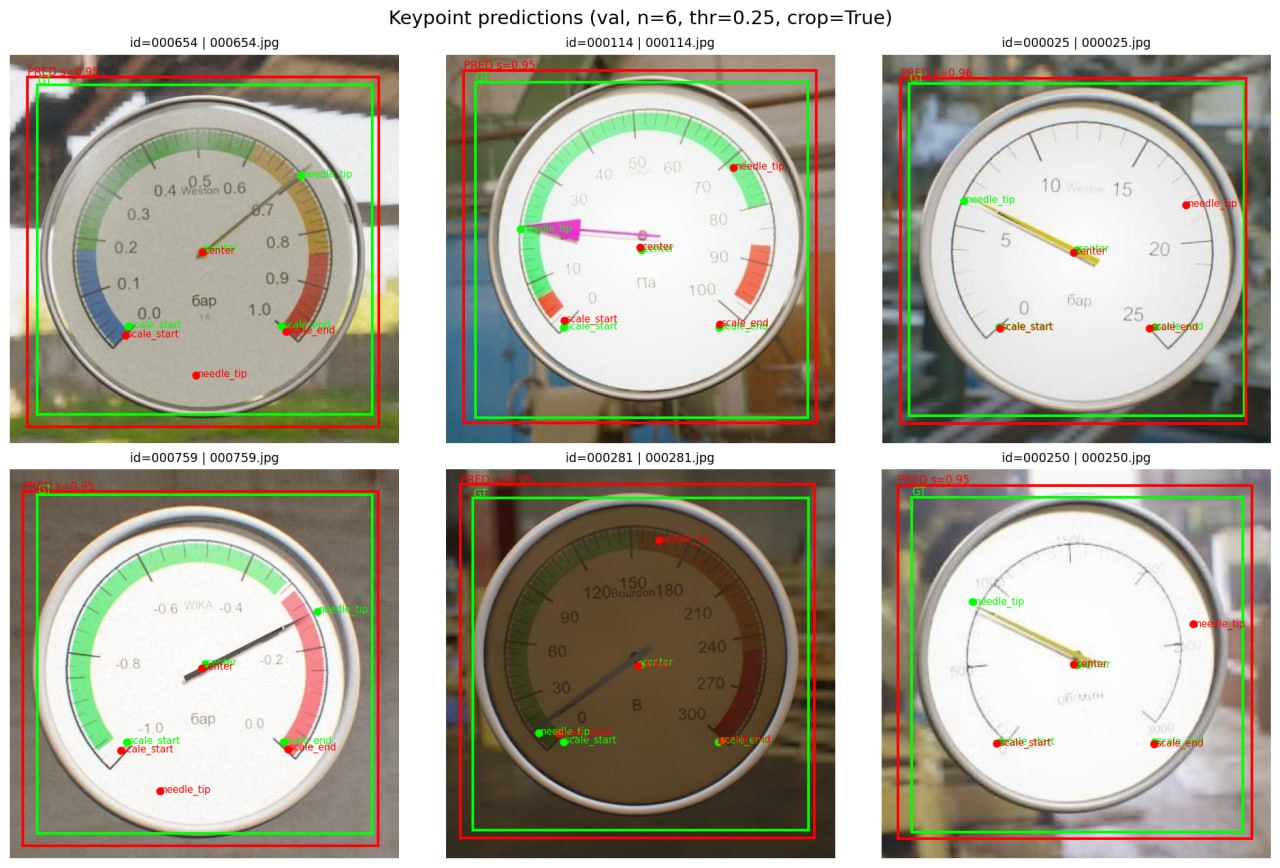
\includegraphics[width=0.90\textwidth]{det_kp_result.jpeg}
			\caption{Примеры работы двухэтапного пайплайна детекции и локализации ключевых точек}
			\label{fig:det_kp_result}
		\end{figure}

	Результаты первого этапа приведены в таблице~\ref{tab:det_results}.

			\begin{table}[htbp]
		\caption{Результаты детекции на тестовой выборке SynthGauge}
		\label{tab:det_results}
		\centering
		\begingroup
		\setstretch{1.0}
		\fontsize{12}{14}\selectfont
		\begin{tabular}{lcccc}
			\toprule
			Модель & Precision & Recall & mAP@0.5 & mAP@0.5:0.95 \\
			\midrule
			YOLOv8n & 0.9864 & 0.9630 & 0.9848 & 0.7803 \\
			\bottomrule
		\end{tabular}
		\endgroup
	\end{table}

	Результаты детекции показывают, что на синтетическом наборе задача локализации циферблата решается очень надежно. Это означает, что ограничивающим фактором пайплайна становится уже не поиск прибора, а точность восстановления его геометрии.

	Результаты второго этапа, связанного с локализацией ключевых точек, приведены в таблице~\ref{tab:kp_results}.

	\begin{table}[htbp]
		\caption{Результаты локализации ключевых точек на тестовой выборке SynthGauge}
		\label{tab:kp_results}
		\centering
		\begingroup
		\setstretch{1.0}
		\fontsize{12}{14}\selectfont
		\setlength{\tabcolsep}{4pt}
			\begin{tabularx}{\textwidth}{>{\raggedright\arraybackslash}p{3.0cm} *{6}{>{\centering\arraybackslash}X}}
				\toprule
				Модель & Pose P & Pose R & mAP@0.5 & mAP50--95 & PCK@0.05 & PCK@0.10 \\
			\midrule
			YOLO11s-pose & 0.9999 & 1.0000 & 0.9950 & 0.6200 & 0.6048 & 0.6665 \\
			\bottomrule
		\end{tabularx}
		\endgroup
	\end{table}

Здесь обозначения $Pose P$ и $Pose R$ соответствуют метрикам $pose\_precision$ и $pose\_recall$.

	Ключевой вывод состоит в том, что геометрический этап заметно труднее этапа локализации прибора. Детектор обычно уверенно находит циферблат, но восстановление ключевых точек требует большей точности: ошибка в положении центра или границ шкалы меняет систему координат, в которой затем считается угол стрелки. Это хорошо согласуется с результатами других работ, где выделение стрелки и восстановление геометрии шкалы рассматриваются как основная проблема интерпретируемого подхода \cite{dyer1983,adsul2021,sciRep2025,linknetYolo2024}.

	\subsection{Эксперимент 2. Сегментация стрелки}

	Следующий этап интерпретируемого пайплайна связан с сегментацией стрелки. Его задача состоит в том, чтобы выделить на обрезанном изображении все пиксели указателя. В отличие от подхода с ключевыми точками, модель не обязана сразу предсказывать единственную точку кончика стрелки. Она строит маску, а уже затем из этой маски вычисляется направление.

		В эксперименте для этого этапа обучается YOLO-seg на crop-изображениях циферблата. Из исходной многоклассовой разметки берется только класс стрелки: он переводится в бинарную маску, затем маска преобразуется в полигональный формат YOLO. При этом исходные бинарные изображения не удаляются, поскольку по ним затем считаются $IoU$, $Dice$ и пиксельные precision/recall.

		Практический смысл сегментации проявляется при разборе ошибок. Лишние пиксели на делениях шкалы обычно ухудшают pixel precision, но не всегда резко меняют угол. Потеря тонкого конца стрелки опаснее: дальние от центра пиксели исчезают из маски, оценка направления смещается к основанию указателя, и итоговое показание может уйти на заметную величину даже при визуально небольшой ошибке.

		Еще одно преимущество маски состоит в том, что она оставляет проверяемый промежуточный результат. На реальном снимке сразу видно, спутала ли модель стрелку с темным делением, захватила ли блик на стекле или потеряла узкий наконечник. Для дальнейшего sim-to-real перехода это важнее, чем просто получить одно число на выходе: ошибка становится локализуемой и ее можно связывать с конкретным визуальным фактором.

		Количественные результаты сегментации на тестовой выборке SynthGauge приведены в таблице~\ref{tab:seg_results}. В таблицу включены метрики, которые непосредственно характеризуют качество выделения стрелки: качество предсказанной маски и пиксельное совпадение с истинной бинарной маской.

	\begin{table}[H]
		\caption{Результаты сегментации стрелки на тестовой выборке SynthGauge}
		\label{tab:seg_results}
		\centering
		\begingroup
		\setstretch{1.0}
		\fontsize{12}{14}\selectfont
			\setlength{\tabcolsep}{2pt}
			\begin{tabularx}{\textwidth}{>{\raggedright\arraybackslash}p{2.6cm} *{8}{>{\centering\arraybackslash}X}}
				\toprule
				Модель & Mask P & Mask R & mAP50 & mAP50--95 & Pixel P & Pixel R & IoU & Dice \\
				\midrule
				YOLO11n-seg & 0.9123 & 0.7978 & 0.8773 & 0.4557 & 0.6915 & 0.7440 & 0.5586 & 0.7168 \\
				\bottomrule
			\end{tabularx}
			\endgroup
		\end{table}

		Здесь $Mask~P$ и $Mask~R$ обозначают precision и recall для маски экземпляра стрелки, $Mask~mAP$ оценивает качество предсказанной маски по порогам $IoU$, а $Pixel~P$, $Pixel~R$, $IoU$ и $Dice$ считаются по бинарной маске стрелки на уровне пикселей.

	На рисунке~\ref{fig:seg_full_samples} показаны примеры работы полного пайплайна с сегментацией стрелки. Визуализация объединяет исходное изображение, найденную область прибора, предсказанную маску стрелки и итоговую геометрическую оценку показания.

	\begin{figure}[p]
		\centering
		\includegraphics[width=\textwidth,height=0.82\textheight,keepaspectratio]{seg_full_samples.png}
		\caption{Демонстрация результатов полного пайплайна с сегментацией стрелки}
		\label{fig:seg_full_samples}
	\end{figure}

	\subsection{Алгоритм получения угла стрелки и показания}

	После детекции, ключевых точек и сегментации требуется перейти от визуальных предсказаний к числу. В полном геометрическом пайплайне используются три опорные точки: центр шкалы $c=(x_c,y_c)$, начало шкалы $s=(x_s,y_s)$ и конец шкалы $e=(x_e,y_e)$. Направление стрелки определяется по маске. Пусть $M$ --- множество пикселей, которые модель отнесла к стрелке. Для каждого пикселя $p=(x_p,y_p)$ считается расстояние до центра:

	\[
		\rho(p) = (x_p - x_c)^2 + (y_p - y_c)^2.
	\]

	Кончик стрелки оценивается как средняя координата небольшой доли самых дальних от центра пикселей маски. В текущей реализации берется примерно 1\% наиболее удаленных пикселей. Это позволяет не зависеть от одного случайного пикселя на краю маски и делает оценку устойчивее к небольшим дефектам сегментации.

	Далее для любой точки $p$ угол относительно центра считается в координатах изображения. Поскольку в изображении ось $y$ направлена вниз, используется не обычная математическая формула угла, а угол по часовой стрелке с нулем сверху:

	\[
		\theta(p) =
		\left(
		\frac{180}{\pi}
		\operatorname{atan2}(x_p - x_c,\, y_c - y_p)
		+ 360
		\right) \bmod 360.
	\]

	По этой формуле вычисляются три угла: $\theta_s=\theta(s)$ для начала шкалы, $\theta_e=\theta(e)$ для конца шкалы и $\theta_n=\theta(n)$ для кончика стрелки. Затем определяется угловой размер основной шкалы:

	\[
		S = (\theta_e - \theta_s) \bmod 360,
	\]

	и прогресс стрелки относительно начала шкалы:

	\[
		P = (\theta_n - \theta_s) \bmod 360.
	\]

	Если стрелка находится внутри дуги шкалы, нормализованное показание получается как

	\[
		\hat{r} = \frac{P}{S}.
	\]

	Значение $\hat{r}=0$ соответствует началу шкалы, а $\hat{r}=1$ --- ее концу. Если вычисленный угол стрелки оказался чуть вне видимой дуги, пайплайн не переносит его через полный круг, а прижимает к ближайшей границе шкалы. Это важно для устойчивости: небольшая ошибка около начала шкалы не должна превращаться в почти максимальное показание только из-за циклической природы углов.

	Такой алгоритм является интерпретируемым. Для каждого предсказания можно отдельно посмотреть crop, ключевые точки, маску стрелки, найденный кончик и итоговый угол. Это делает его удобным для анализа ошибок и для будущего промышленного внедрения, где пользователю важно не только получить число, но и понимать, почему система решила именно так.

	\subsection{Эксперимент 3. Прямая регрессия показания}

	В регрессионном подходе задача решается напрямую как предсказание нормализованного показания по изображению циферблата. В качестве базовой модели используется ResNet-18. В отличие от геометрического пайплайна, этот подход не восстанавливает геометрию явно, а сразу переводит изображение в числовое значение \cite{leon2024,meterRegression2024,sciRep2025}.

На рисунке~\ref{fig:regression_result} показаны примеры работы регрессионной модели. В большинстве случаев предсказания близки к истинным значениям, однако сам механизм ошибки здесь менее прозрачен.

Для оценки качества используются $MAE$, $RMSE$, $R^2$ и $DRR@0.02$. Результаты отражены в таблице~\ref{tab:reg_results}.

	\begin{table}[htbp]
		\caption{Результаты прямой регрессии на тестовой выборке SynthGauge}
		\label{tab:reg_results}
		\centering
		\begingroup
		\setstretch{1.0}
		\fontsize{12}{14}\selectfont
		\begin{tabular}{lcccc}
			\toprule
			Модель & $MAE$ & $DRR@0.02$ & $RMSE$ & $R^2$ \\
			\midrule
			ResNet-18 & 0.0182 & 0.6970 & 0.0372 & 0.9819 \\
			\bottomrule
		\end{tabular}
		\endgroup
	\end{table}

	Полученные значения показывают, что модель способна достаточно точно предсказывать показание без явной геометрической постобработки. Одновременно такой подход хуже интерпретируется и потенциально сильнее зависит от доменного сдвига \cite{meterRegression2024,zhang2019,sciRep2025}.

			\begin{figure}[htbp]
				\centering
				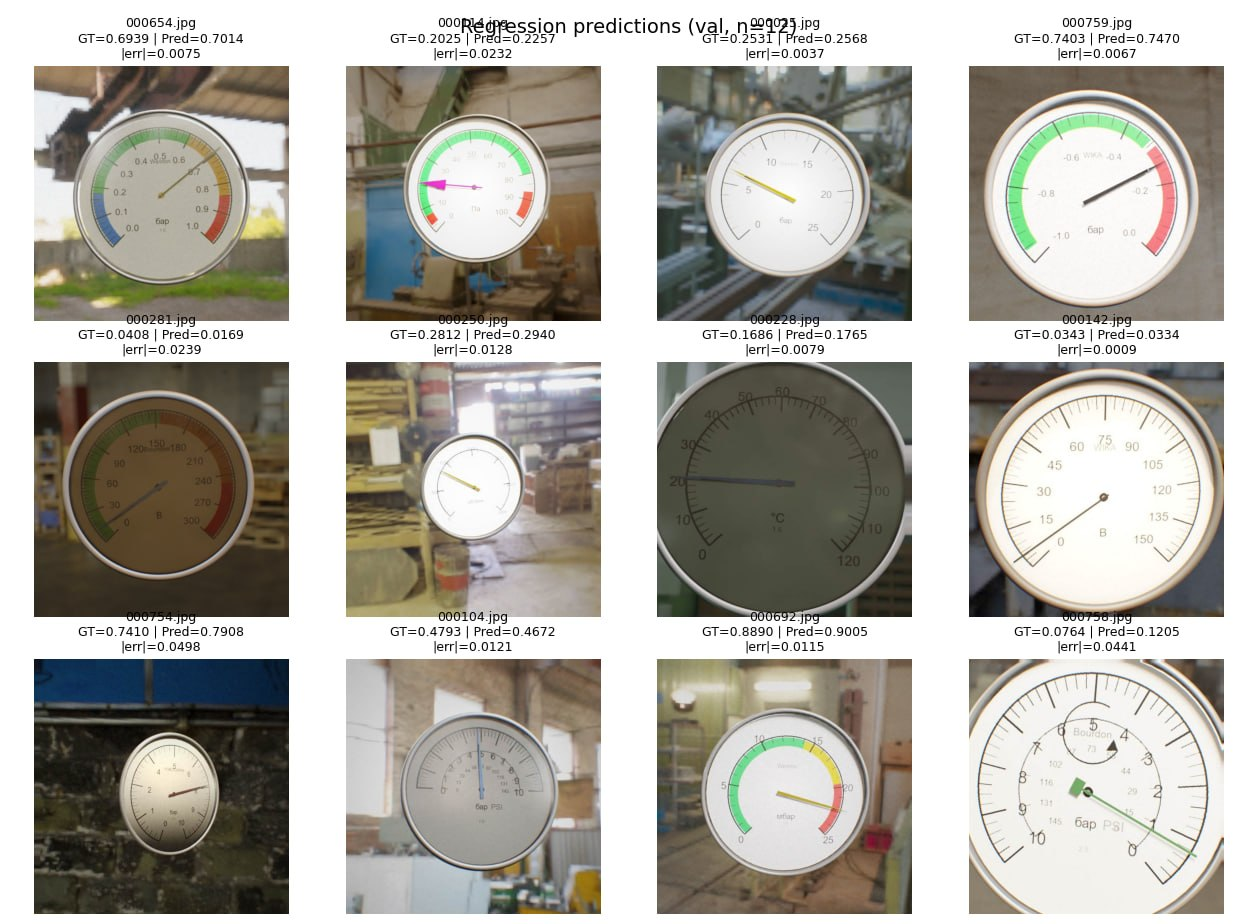
\includegraphics[width=0.82\textwidth,height=0.34\textheight,keepaspectratio]{regression_result.jpeg}
				\caption{Примеры предсказаний модели прямой регрессии на изображениях датчиков}
				\label{fig:regression_result}
			\end{figure}

	\subsection{Тест на реальных данных}

	Отдельная проверка выполнена для реальных изображений с landmark-разметкой. В отличие от синтетического набора, реальные данные не содержат такой же полной семантической маски стрелки, поэтому эксперимент не является полностью симметричным синтетическому тесту. Для реальных изображений используются категории, соответствующие центру прибора, минимуму шкалы, максимуму шкалы, кончику стрелки и самому прибору. Истинное нормализованное показание для такого набора можно получить геометрически: по разметке центра, начала и конца шкалы, а также по разметке кончика стрелки.

	Этот тест важен именно как проверка переноса, а не как финальная демонстрация промышленной готовности. На синтетических изображениях модели видят распределение, близкое к обучающему: похожие материалы, ракурсы, разметку и типы шкал. Реальные фотографии отличаются сильнее. Там появляются неидеальные углы съемки, неравномерное освещение, стеклянные блики, низкое разрешение, частично закрытые циферблаты, фоновые объекты и приборы, которые не совпадают с синтетическими шаблонами.

	Качественная проверка показывает, что отдельные элементы пайплайна переносятся на реальные изображения, но пока не идеально. Детекция прибора часто остается наиболее устойчивым этапом: если прибор хорошо виден и занимает заметную часть кадра, модель обычно способна найти область циферблата. Основные проблемы возникают дальше. Ключевые точки могут смещаться на шкалах с нестандартным расположением делений, а сегментация стрелки может путать стрелку с темными делениями, бликами или декоративными элементами. В результате итоговое показание иногда оказывается правдоподобным, но в других случаях ошибка становится заметной.

	На рисунке~\ref{fig:full_pipeline_real_landmarks_samples} приведены примеры работы пайплайна на реальных фотографиях с landmark-разметкой. Эти примеры показывают, какие элементы контура переносятся с синтетики на реальные изображения, а где появляются ошибки из-за отличий освещения, фона и внешнего вида приборов.

	\begin{figure}[p]
		\centering
		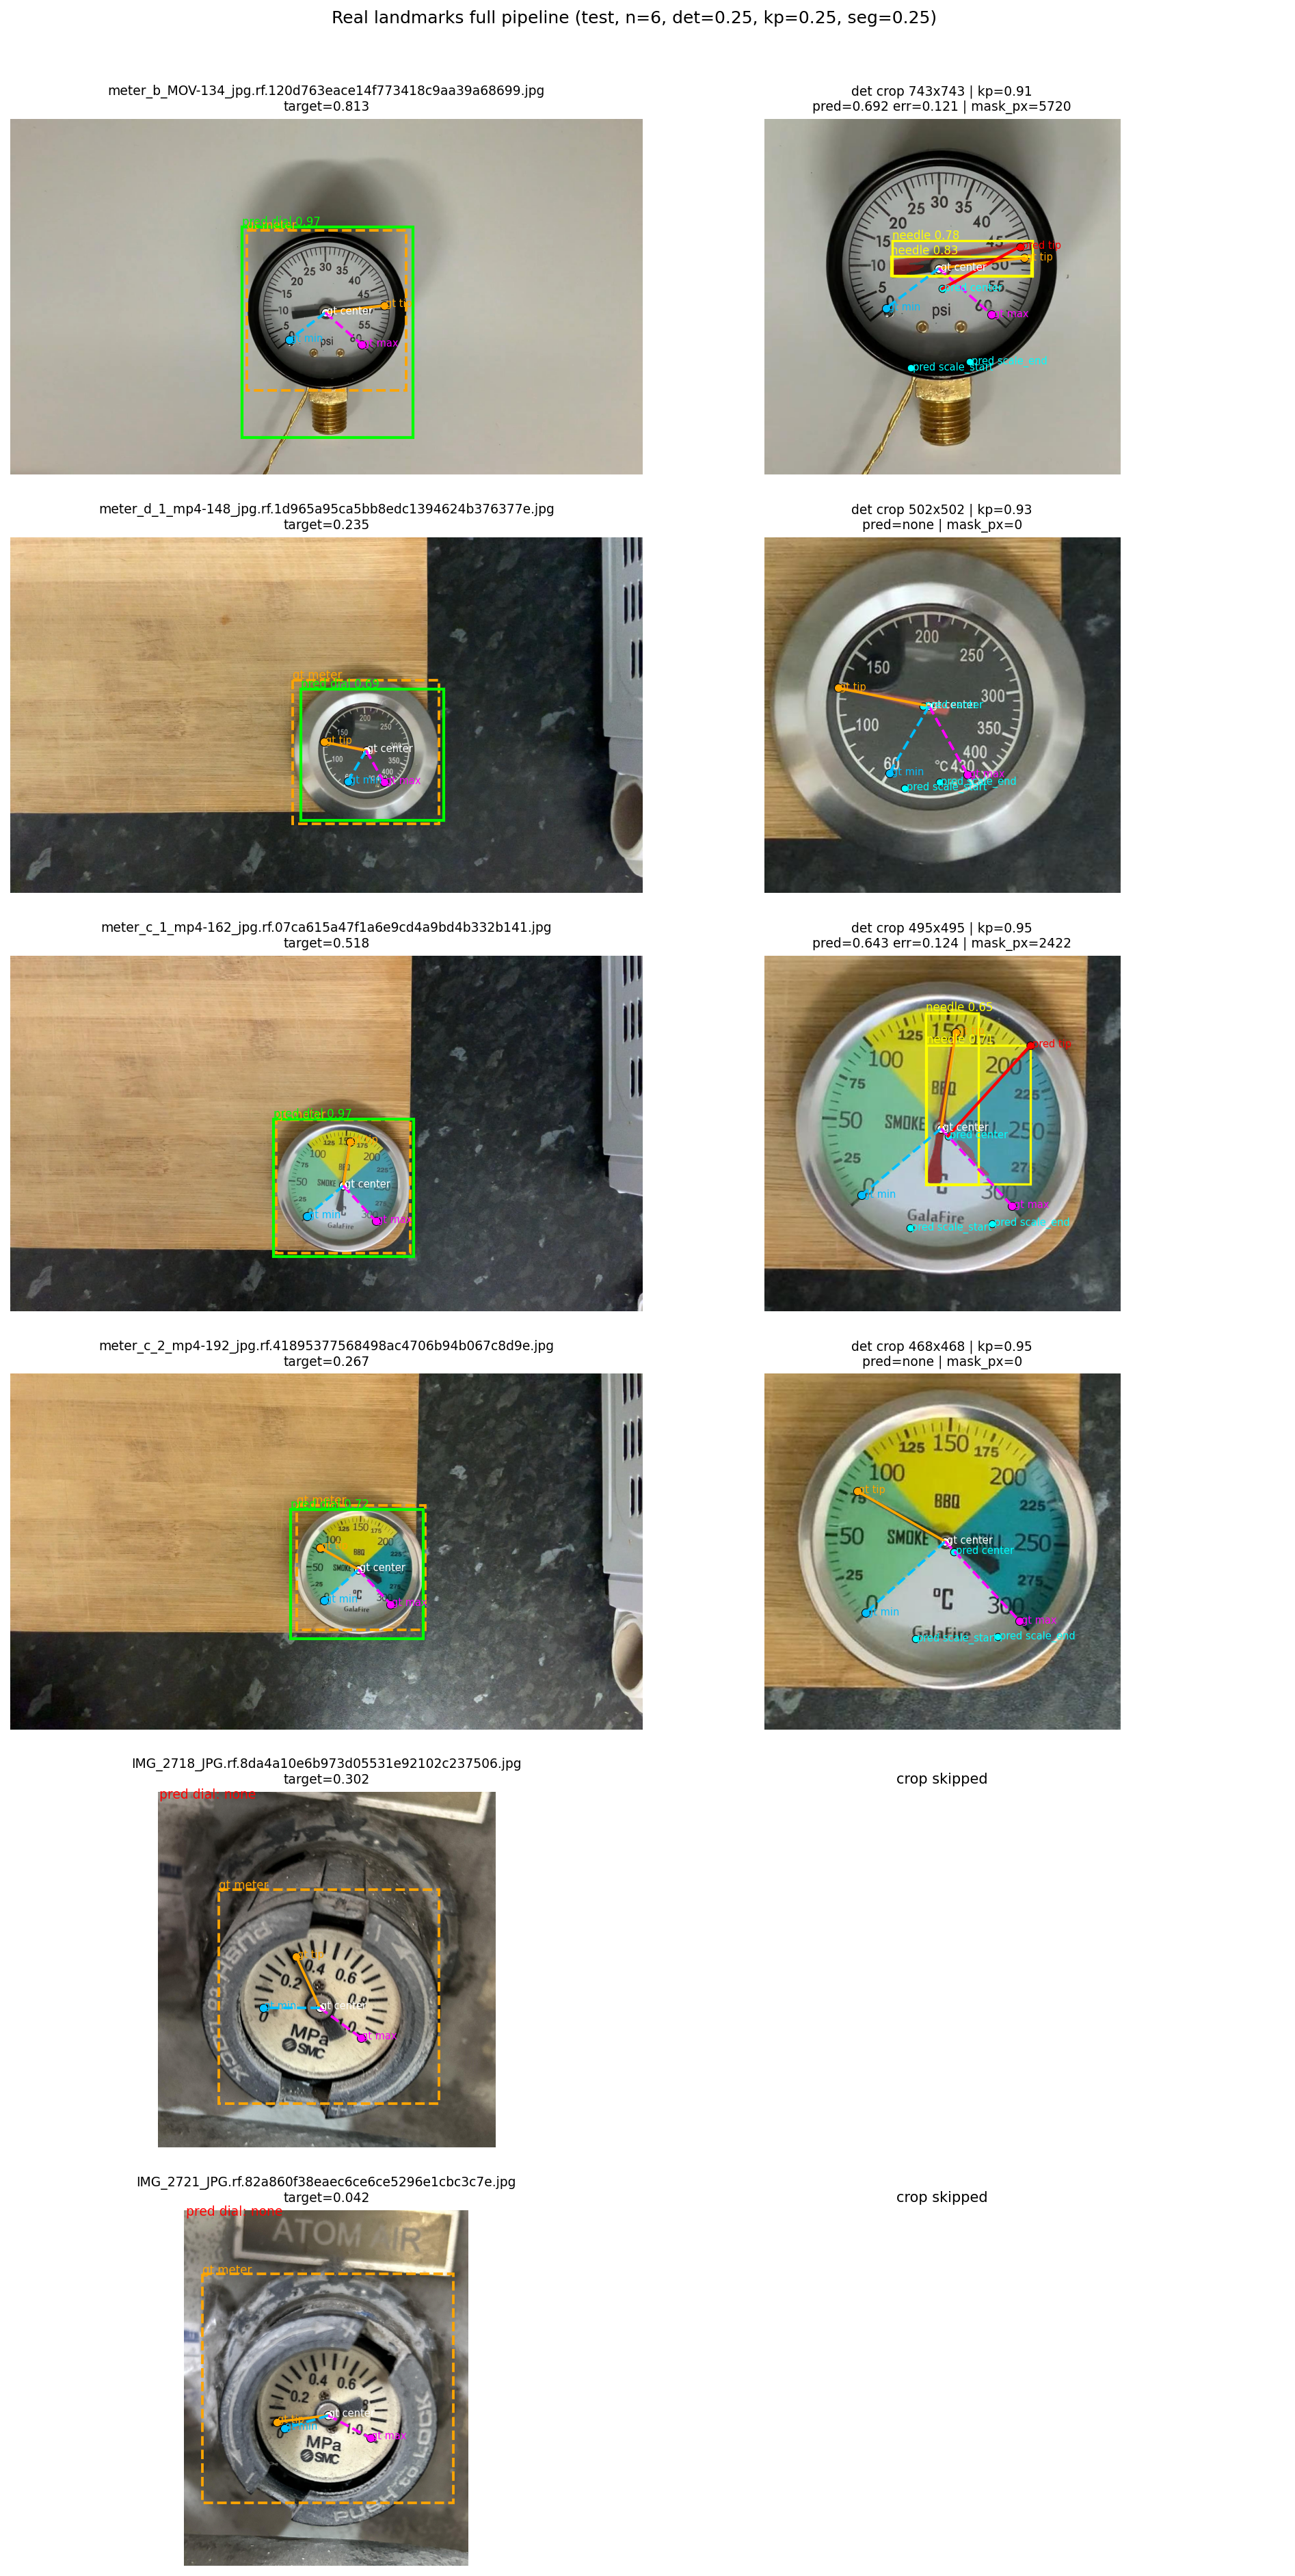
\includegraphics[width=\textwidth,height=0.82\textheight,keepaspectratio]{full_pipeline_real_landmarks_samples.png}
		\caption{Демонстрация работы пайплайна на реальных изображениях с landmark-разметкой}
		\label{fig:full_pipeline_real_landmarks_samples}
	\end{figure}

	Численные результаты полного геометрического пайплайна с сегментацией приведены в таблице~\ref{tab:full_pipeline_results}. Для сопоставления показаны результаты на синтетической тестовой выборке и на реальных изображениях. На реальных данных истинные маски стрелки отсутствуют, поэтому $IoU$ сегментации для этого набора не рассчитывается.

	\begin{table}[htbp]
		\caption{Результаты полного пайплайна с сегментацией на синтетических и реальных данных}
		\label{tab:full_pipeline_results}
		\centering
		\begingroup
		\setstretch{1.0}
		\fontsize{12}{14}\selectfont
		\begin{tabularx}{\textwidth}{>{\raggedright\arraybackslash}X >{\centering\arraybackslash}p{3.2cm} >{\centering\arraybackslash}p{3.2cm}}
			\toprule
			Метрика & SynthGauge test & Реальные изображения \\
			\midrule
			Число изображений & 1000 & 150 \\
			Валидные считывания & 951 & 74 \\
			Покрытие считывания & 0.9510 & 0.4933 \\
			\midrule
			$MAE$ показания & 0.0539 & 0.1525 \\
			$Acc@5\%$ & 0.7610 & 0.1800 \\
			Ошибка ключевых точек & 0.0374 & 0.0822 \\
			Ошибка ключевых точек, px & 10.59 & 60.00 \\
			$IoU$ сегментации стрелки & 0.5743 & -- \\
			$MAE$ угла стрелки, град. & 7.94 & 30.15 \\
			\midrule
			Доля найденных приборов & 1.0000 & 0.8133 \\
			Доля найденных ключевых точек & 0.9910 & 0.6733 \\
			Доля найденных масок стрелки & 0.9600 & 0.5733 \\
			\bottomrule
		\end{tabularx}
		\endgroup
	\end{table}

	Текущий пайплайн пока нельзя считать готовым промышленным решением для произвольных реальных фотографий. Его сильная сторона состоит в том, что он дает понятную структуру ошибки. Если на реальном изображении неверно выделена стрелка, это видно по маске. Если неверно найдены границы шкалы, это видно по ключевым точкам. Это лучше, чем ситуация с прямой регрессией, где модель может дать неверное число без объяснимого промежуточного состояния.

	\begin{table}[htbp]
		\caption{Качественные наблюдения на реальных изображениях}
		\label{tab:real_qualitative}
		\centering
		\begingroup
		\setstretch{1.0}
		\fontsize{12}{14}\selectfont
		\begin{tabularx}{\textwidth}{>{\raggedright\arraybackslash}p{3.3cm} X X}
			\toprule
			Компонент & Преимущества & Недостатки \\
			\midrule
			Детекция & Находит крупные и хорошо видимые приборы & Ошибается при частичном перекрытии, сложном фоне и малом размере прибора \\
			Ключевые точки & Устойчива на простых круглых шкалах & Смещается на нестандартных шкалах, при бликах и низком контрасте \\
			Сегментация стрелки & Позволяет визуально проверить направление указателя & Может захватывать деления шкалы или терять тонкий конец стрелки \\
			Итоговое считывание & Иногда дает правдоподобное значение без ручного вмешательства & Пока нестабильно для полностью автономного применения \\
			\bottomrule
		\end{tabularx}
		\endgroup
	\end{table}

	Главный вывод из теста на реальных данных заключается в том, что синтетическое обучение дает полезную стартовую точку, но само по себе не закрывает задачу sim-to-real. Для улучшения качества нужны либо реальные доразмеченные изображения, либо более агрессивная доменная рандомизация, либо адаптация модели на небольшом наборе фотографий с целевого производства. Для малых заводов это все равно может быть практичным сценарием: требуется не полная замена оборудования, а сбор ограниченного набора фотографий уже установленных приборов и донастройка модели под конкретные условия съемки.

	\subsection{Сравнительный анализ результатов}

	Сопоставление подходов позволяет сделать несколько выводов. Во-первых, локализация самого прибора на синтетических данных уже не является главным ограничением. Во-вторых, внутри интерпретируемого пайплайна узким местом остается восстановление геометрии: нужно одновременно правильно найти центр, границы шкалы и направление стрелки. Сегментация стрелки делает этот этап более содержательным, потому что позволяет использовать всю форму указателя, а не только одну точку.

	В-третьих, по имеющимся численным результатам на синтетическом тесте наиболее качественным методом остается прямая регрессия. Значение $MAE=0.0182$ означает, что средняя ошибка составляет около 1.8\% от нормированного диапазона шкалы, а $R^2=0.9819$ указывает на сильное соответствие предсказаний истинным значениям. Если оценивать только синтетический тестовый набор и только конечное число, этот подход выглядит лучшим.

		Однако для реального внедрения вывод сложнее. Прямая регрессия является менее прозрачной: если она ошиблась, трудно понять, увидела ли модель неверную стрелку, перепутала шкалу или просто столкнулась с незнакомым визуальным стилем. Интерпретируемый пайплайн с сегментацией пока уступает по зрелости, но лучше подходит для диагностики и постепенного улучшения. Поэтому текущий итог можно сформулировать так: лучшим по численной синтетической метрике является регрессионный подход, а наиболее перспективным для промышленного развития является гибридный геометрический пайплайн с детекцией, ключевыми точками и сегментацией стрелки.

	\subsection{Ограничения текущей реализации и план доработки}

	Из полученных результатов можно сформулировать следующие ограничения:

\begin{enumerate}[leftmargin=1.5cm]
		\item Основные численные результаты получены на синтетическом наборе данных; перенос на реальные изображения пока не является стабильным.
		\item Интерпретируемый пайплайн чувствителен к ошибкам ключевых точек и маски стрелки, поскольку итоговое показание вычисляется из геометрии.
		\item Реальные изображения часто отличаются от синтетических по освещению, фону, качеству съемки и внешнему виду приборов.
		\item Прямая регрессия показывает сильный результат на синтетике, но хуже подходит для анализа причин ошибки.
	\end{enumerate}

Исходя из этого, направления дальнейшей доработки звучат так:

\begin{enumerate}[leftmargin=1.5cm]
		\item Расширить набор реальных изображений и добавить разметку, достаточную для проверки полного пайплайна, включая маску стрелки.
		\item Улучшить доменную рандомизацию синтетического генератора: добавить больше бликов, загрязнений, неидеальных ракурсов, низкого разрешения и реальных фоновых условий.
			\item Сравнить прямую регрессию с полным геометрическим пайплайном не только на синтетике, но и на небольшом наборе реальных приборов \cite{wang2022,coords2023,meterRegression2024}.
			\item Исследовать гибридный подход, в котором геометрический пайплайн дает интерпретируемую оценку, а регрессия используется как дополнительная проверка или корректор.
			\item Исследовать возможности облегчения модели и ее дальнейшего промышленного внедрения, включая квантование, использование более компактных архитектур и воспроизводимые MLOps-конвейеры \cite{quantization2021,mobilenetv2,lightweightInspection2024,mlops2023}.
			\item Поддерживать воспроизводимость экспериментов через открытый репозиторий с кодом проекта \cite{gaugesReaderRepo2026}.

		\end{enumerate}

	\subsection{Вывод по практической части}

		Результаты экспериментов показывают, что реализованный пайплайн уже задает хорошую основу для дальнейшей работы. Его сильная сторона состоит в том, что отдельные компоненты задачи не смешиваются в один неинтерпретируемый блок: детекция, ключевые точки, сегментация стрелки, геометрический расчет и регрессия могут анализироваться отдельно. На текущем синтетическом тесте наиболее качественный итоговый численный результат показывает прямая регрессия. В то же время для реального промышленного применения более перспективным выглядит интерпретируемый контур с сегментацией стрелки, потому что он позволяет видеть источник ошибки и постепенно адаптировать систему под конкретные приборы.

		Практический вывод особенно важен для малых производств. Уже сейчас можно рассматривать подобный подход как технологию мягкой цифровизации: не заменять всю измерительную цепочку, а добавить визуальное считывание поверх существующих аналоговых приборов. Полностью автономным решением текущую систему считать рано, особенно на реальных изображениях. Но как исследовательская и инженерная база для дальнейшей адаптации она показывает понятное направление развития: собрать небольшой набор реальных фотографий, донастроить модели под целевой объект, сохранить интерпретируемую геометрию и использовать регрессию как сильный базовый ориентир для сравнения.

	\newpage
	\section{Заключение}

		В работе была собрана и проверена схема считывания круглых аналоговых шкал по изображению. В качестве практического сценария выбран случай, когда на объекте уже стоят исправные стрелочные приборы, а цифровой мониторинг нужно добавить без быстрой замены всей измерительной инфраструктуры. Поэтому основной акцент сделан на визуальном считывании: прибор остается на месте, а алгоритм работает с фотографией циферблата.

		В теоретической части были сопоставлены геометрические методы, модели ключевых точек, сегментация стрелки и прямая регрессия. В практической части эти постановки сведены к одному экспериментальному контуру на SynthGauge: из одного набора разметки подготовлены данные для детекции, pose-задачи, сегментации и регрессии нормализованного показания.

		Результаты показали, что поиск самого циферблата на синтетике уже не является главным ограничением: для YOLOv8n получено $mAP@0.5=0.9848$. Сложность переносится внутрь прибора. Модель ключевых точек дала $PCK@0.05=0.6048$, то есть ошибка в центре или границах шкалы остается заметной для последующего расчета угла. Сегментация стрелки помогает увидеть форму указателя и источник сбоя, но качество маски пока также ограничивает итоговый геометрический пайплайн.

		На синтетическом тесте лучшим по конечной численной ошибке оказался ResNet-18: $MAE=0.0182$, $RMSE=0.0372$, $R^2=0.9819$. Этот результат полезен как сильный ориентир, но он почти не объясняет, почему конкретное предсказание ошиблось. Геометрический вариант с сегментацией проигрывает по метрике на SynthGauge, зато оставляет проверяемые промежуточные объекты: рамку, ключевые точки, маску стрелки и рассчитанный угол.

		Отдельная проверка на реальных фотографиях показала масштаб sim-to-real разрыва. Полный пайплайн на SynthGauge test дал $MAE=0.0539$ и $Acc@5\%=0.7610$, а на реальных изображениях --- $MAE=0.1525$ и $Acc@5\%=0.1800$. Такой результат не позволяет называть систему готовой к автономному промышленному применению. Зато он показывает, какие этапы нужно усиливать: устойчивость ключевых точек, выделение стрелки и адаптацию под реальные условия съемки.

		Следующий шаг видится не в усложнении одной модели, а в работе с доменом применения: собрать небольшой набор реальных снимков целевых приборов, доразметить центр, границы шкалы и стрелку, а затем дообучить компоненты пайплайна. Перспективным также остается гибридный вариант, где регрессия используется как сильный численный ориентир, а геометрический контур сохраняет объяснимость и помогает разбирать ошибки на конкретном объекте.

	\newpage
	\printbibliography[heading=bibintoc]

\end{document}
